\subsection{\nnh Event Selection}
The \nnh channel includes $ZH$ production followed by invisible $Z-$decay, or $t-$channel $W-$fusion process. 
The dominant backgrounds are quark pair production and gauge boson pair production, followed by hadronic and invisible decay of each boson. 
The observable particles in the signal form two energetic jets, initiated from two quarks of higgs decay. 
Thus isolation leptons are rejected, and a minimum number of PFOs are required the quark pair. 
The signal events are featured in the kinematic distribution of invisible section.  
The visible energy of the signal events are significantly lower than reducible SM backgrounds like semi-leptonic $WW$ events. 
The visible transverse momentum are required to larger than 19 \GeV to reject \qq events, which tend to have low visible tranverse momentum due to 
high fraction of radiation return events.
The invariant mass of the jets characterize the higgs production which is obverse discriminator against the non-higgs production SM events
\footnote{The peak of in signal region of \qq events is due to radiation events.}.
The angle between two jets and $y$-th values are also useful to distinguish signal events from SM backgrounds.  
Meanwhile the recoil system of these two jets, which is not directly observable, has the charaterstic of the $Z$ boson associate with higgs in final states. The distribution of the above varibles and cut value can be found in figure \ref{fig:kinematic_nnh} and \ref{fig:yth_nnh} for signal and background events. \par

The Boost decision tree \cite{BDT} method is implemented to the survived events from cut chain. The variables used 
in BDT are mentioned aboved: visible energy,  transverse momentum, $y-th$ value, jet pair recoil and invariant mass. 
The events yields of signal and background in cutflow and BDT selection can be found in table \ref{tab:nnh_cut}. \par


\begin{figure}[!htbp]
\label{fig:kinematic_nnh}
\centering
\subfigure[]
{
  \begin{minipage}[b]{0.31\textwidth}
  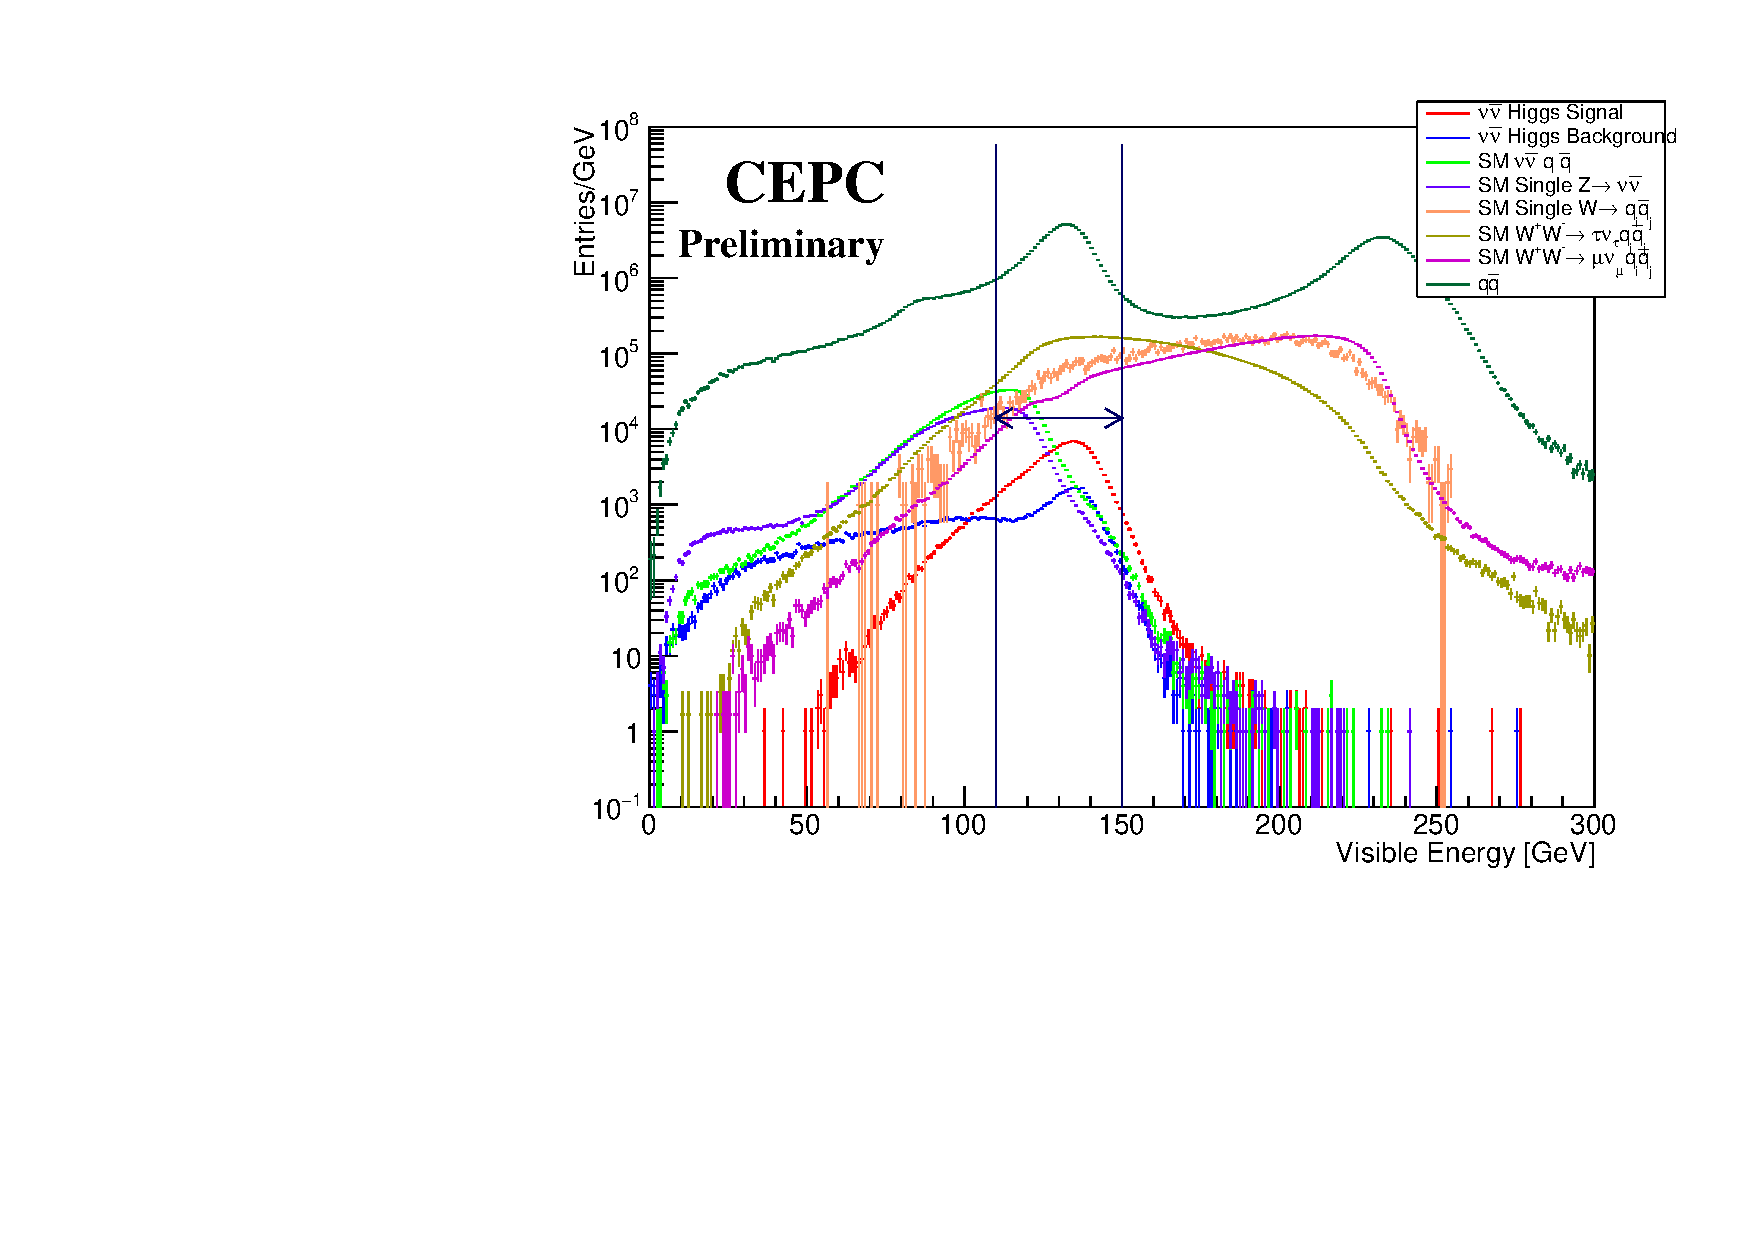
\includegraphics[width=\textwidth]{Analysis/nnh/Etot.pdf}
  \end{minipage}
}
\subfigure[]
{
  \begin{minipage}[b]{0.31\textwidth}
  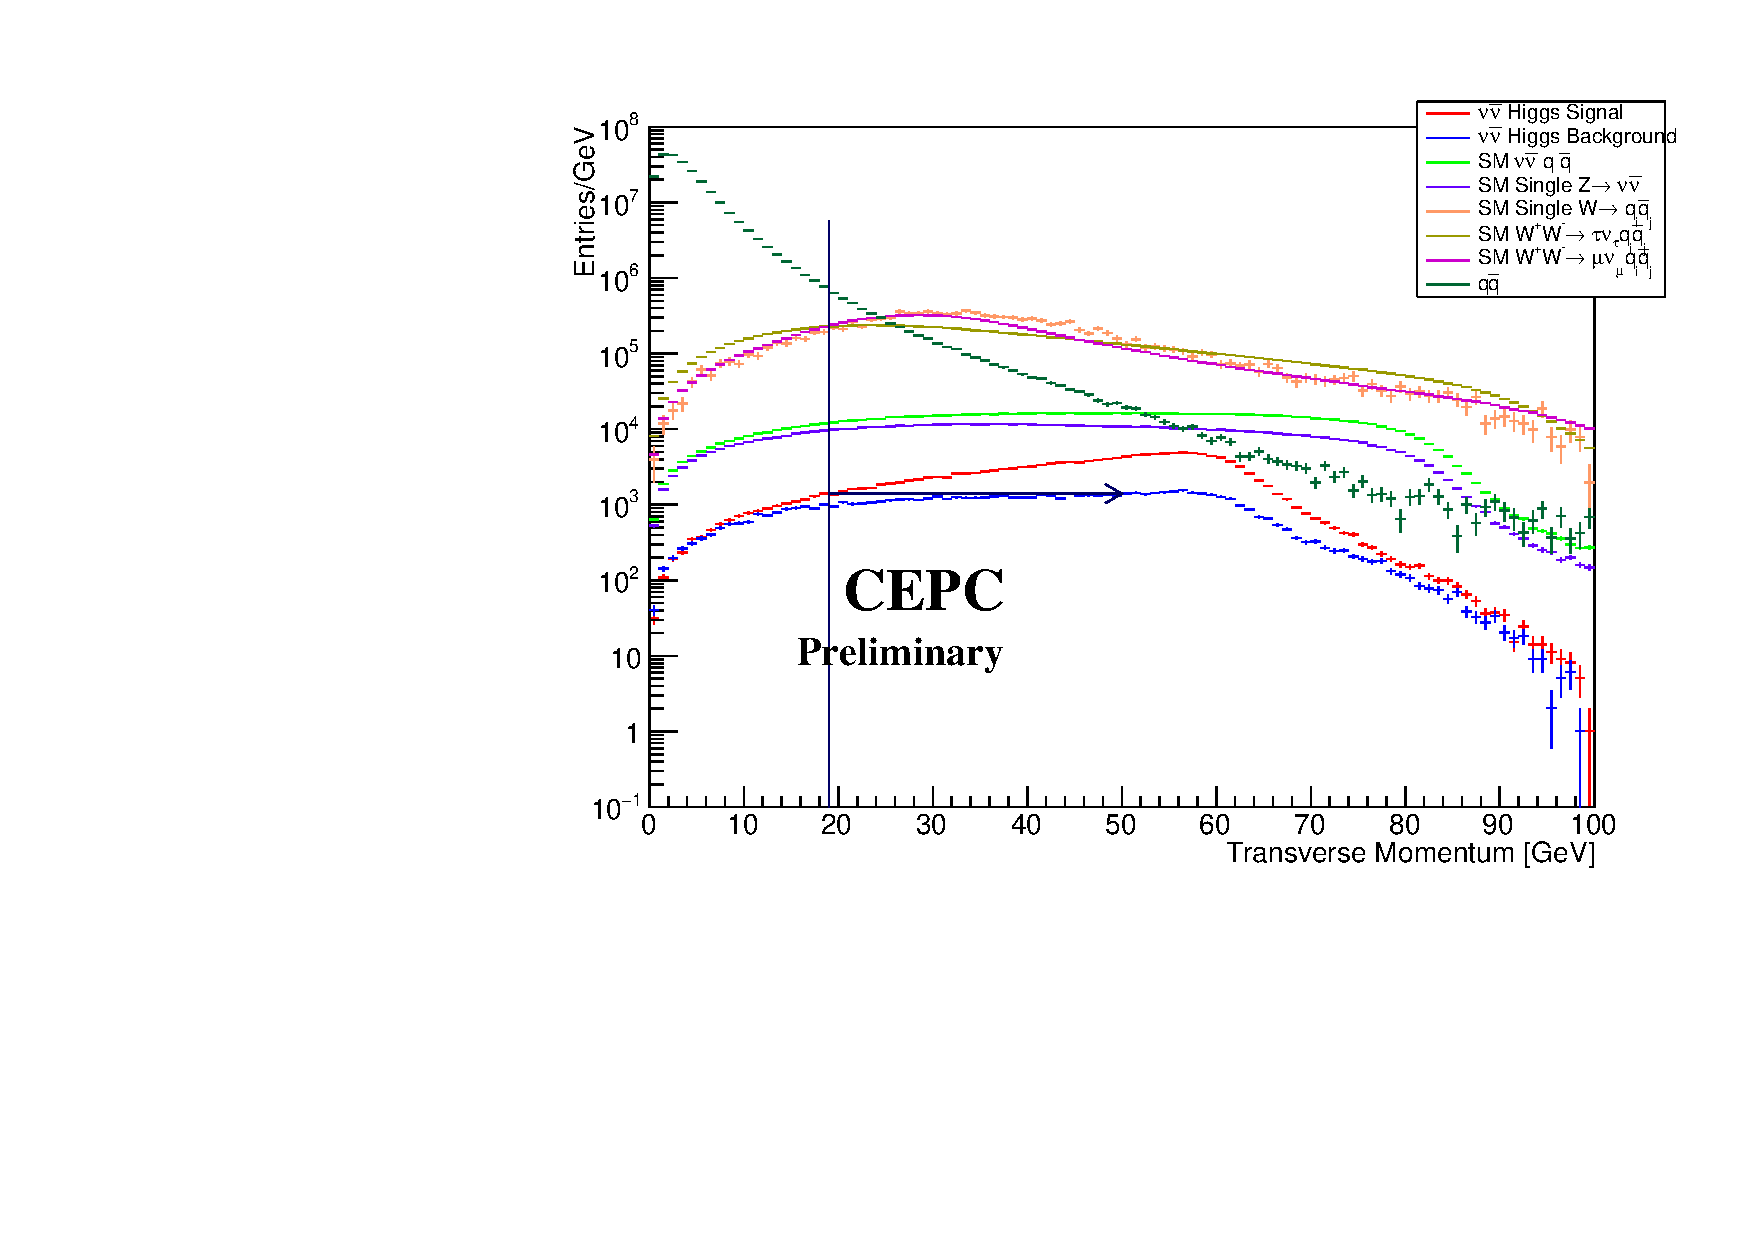
\includegraphics[width=\textwidth]{Analysis/nnh/pT.pdf}
  \end{minipage}
}
\subfigure[]
{
  \begin{minipage}[b]{0.31\textwidth}
  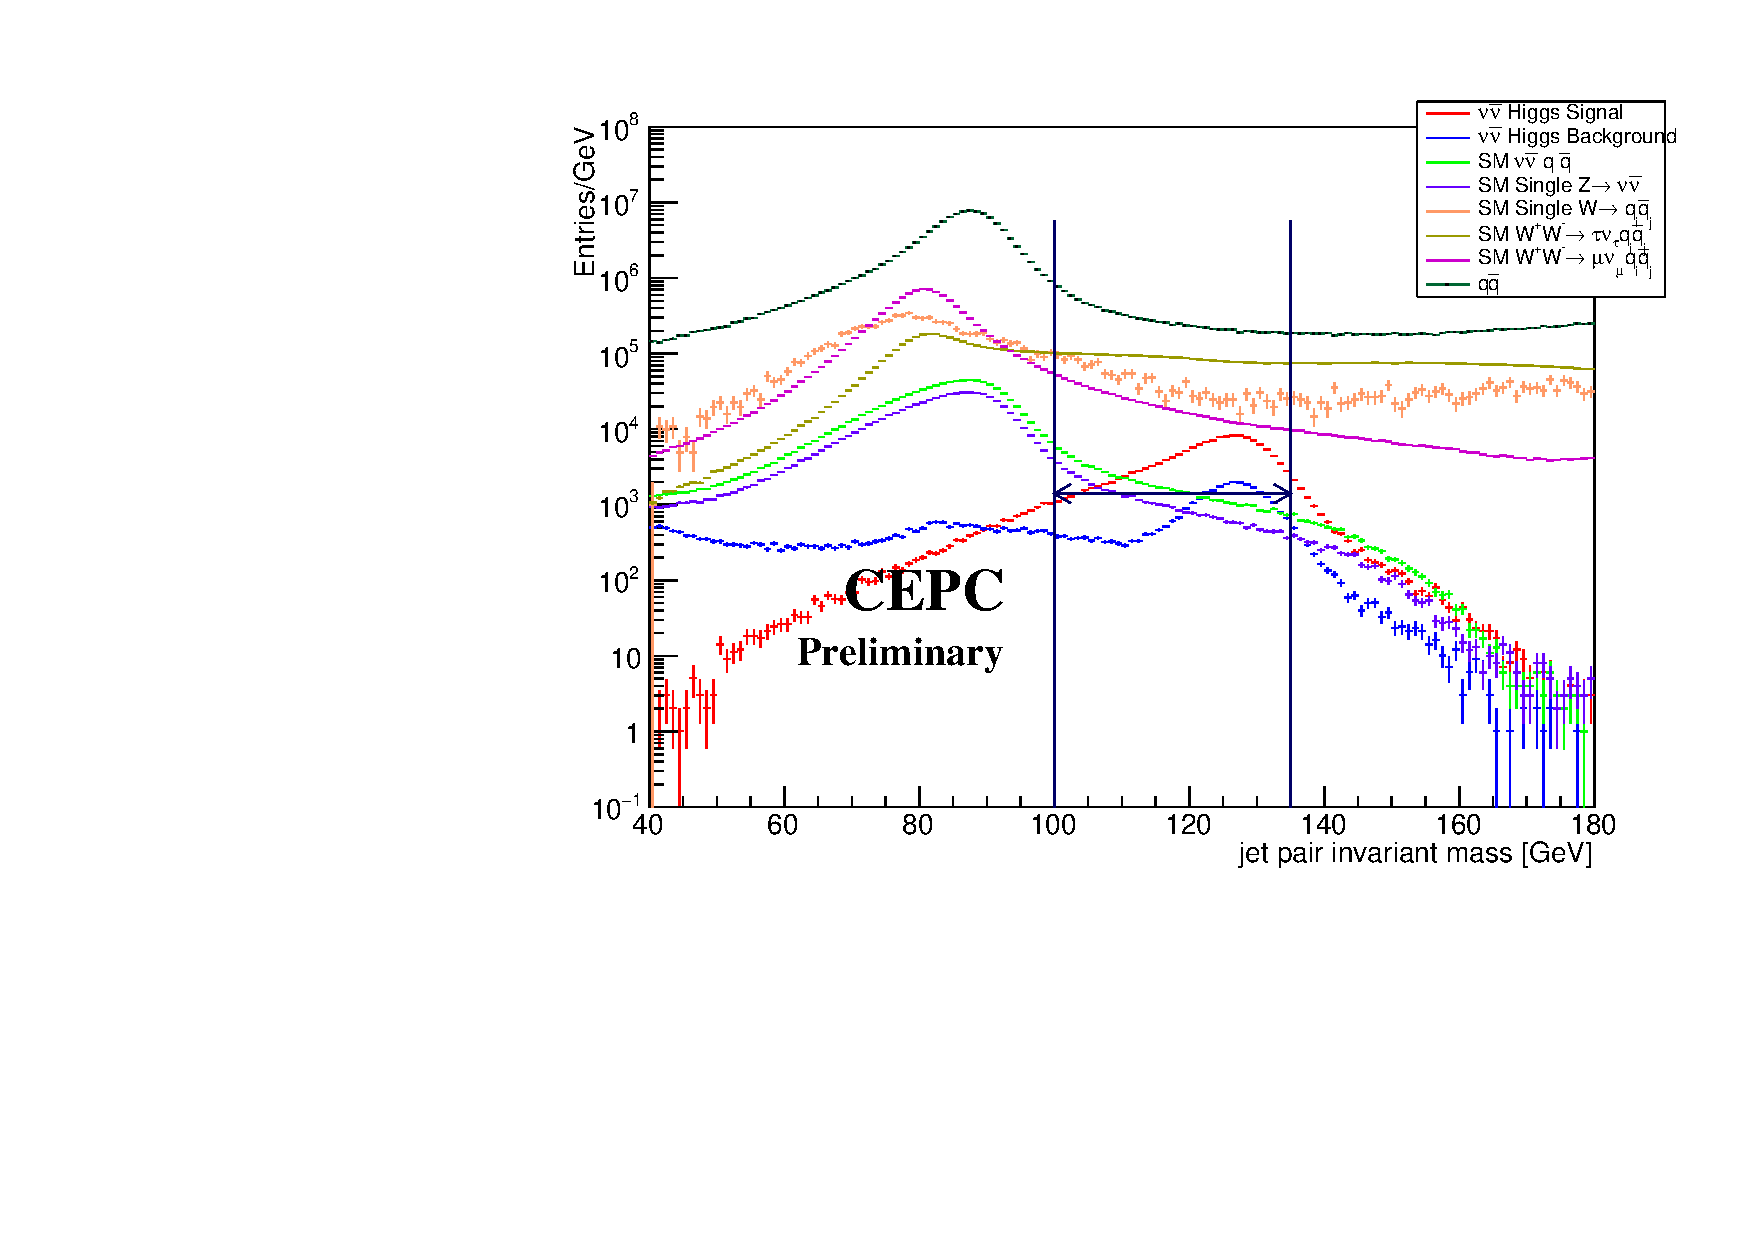
\includegraphics[width=\textwidth]{Analysis/nnh/jj_inv.pdf}
  \end{minipage}
}
\subfigure[]
{ 
   \begin{minipage}[b]{0.31\textwidth}
   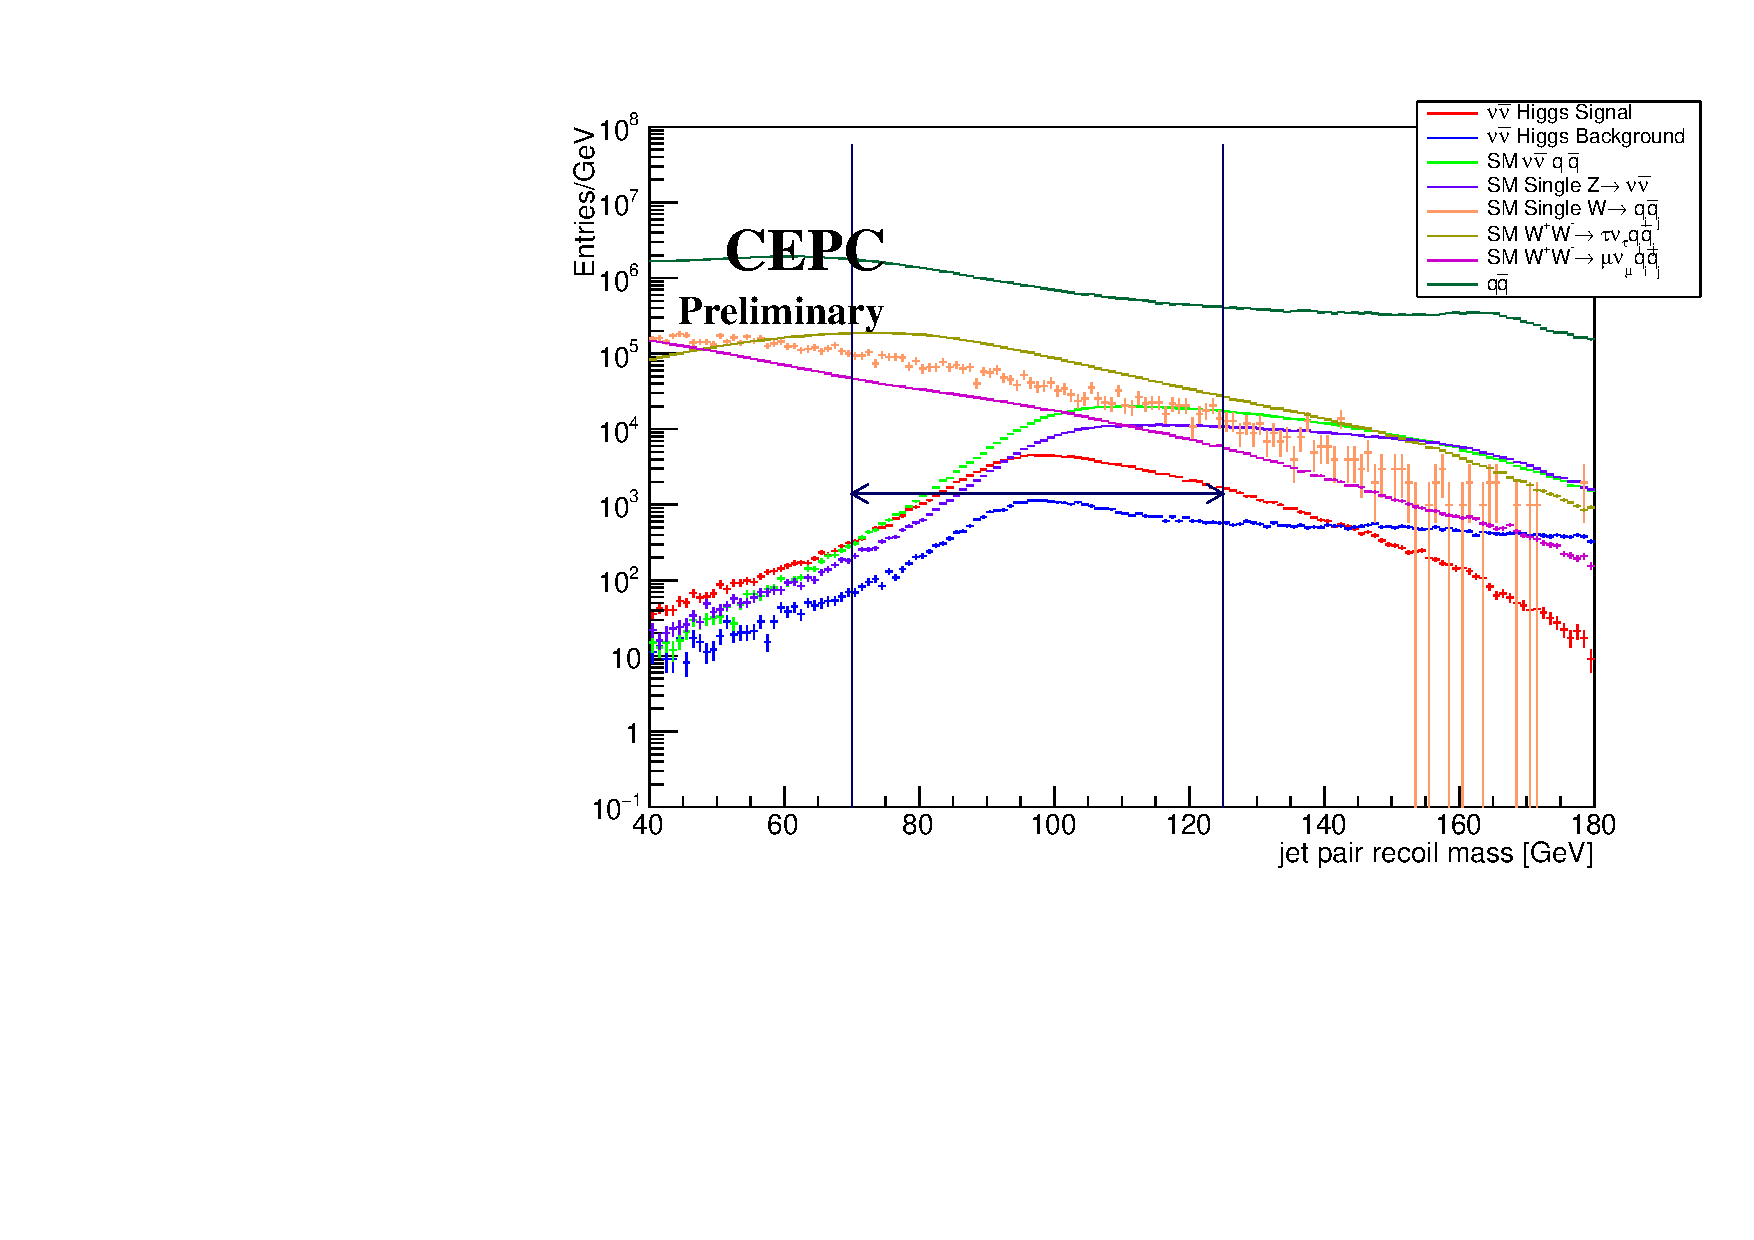
\includegraphics[width=\textwidth]{Analysis/nnh/jj_recoil.pdf}
   \end{minipage}
}
\subfigure[]
{
    \begin{minipage}[b]{0.31\textwidth}
    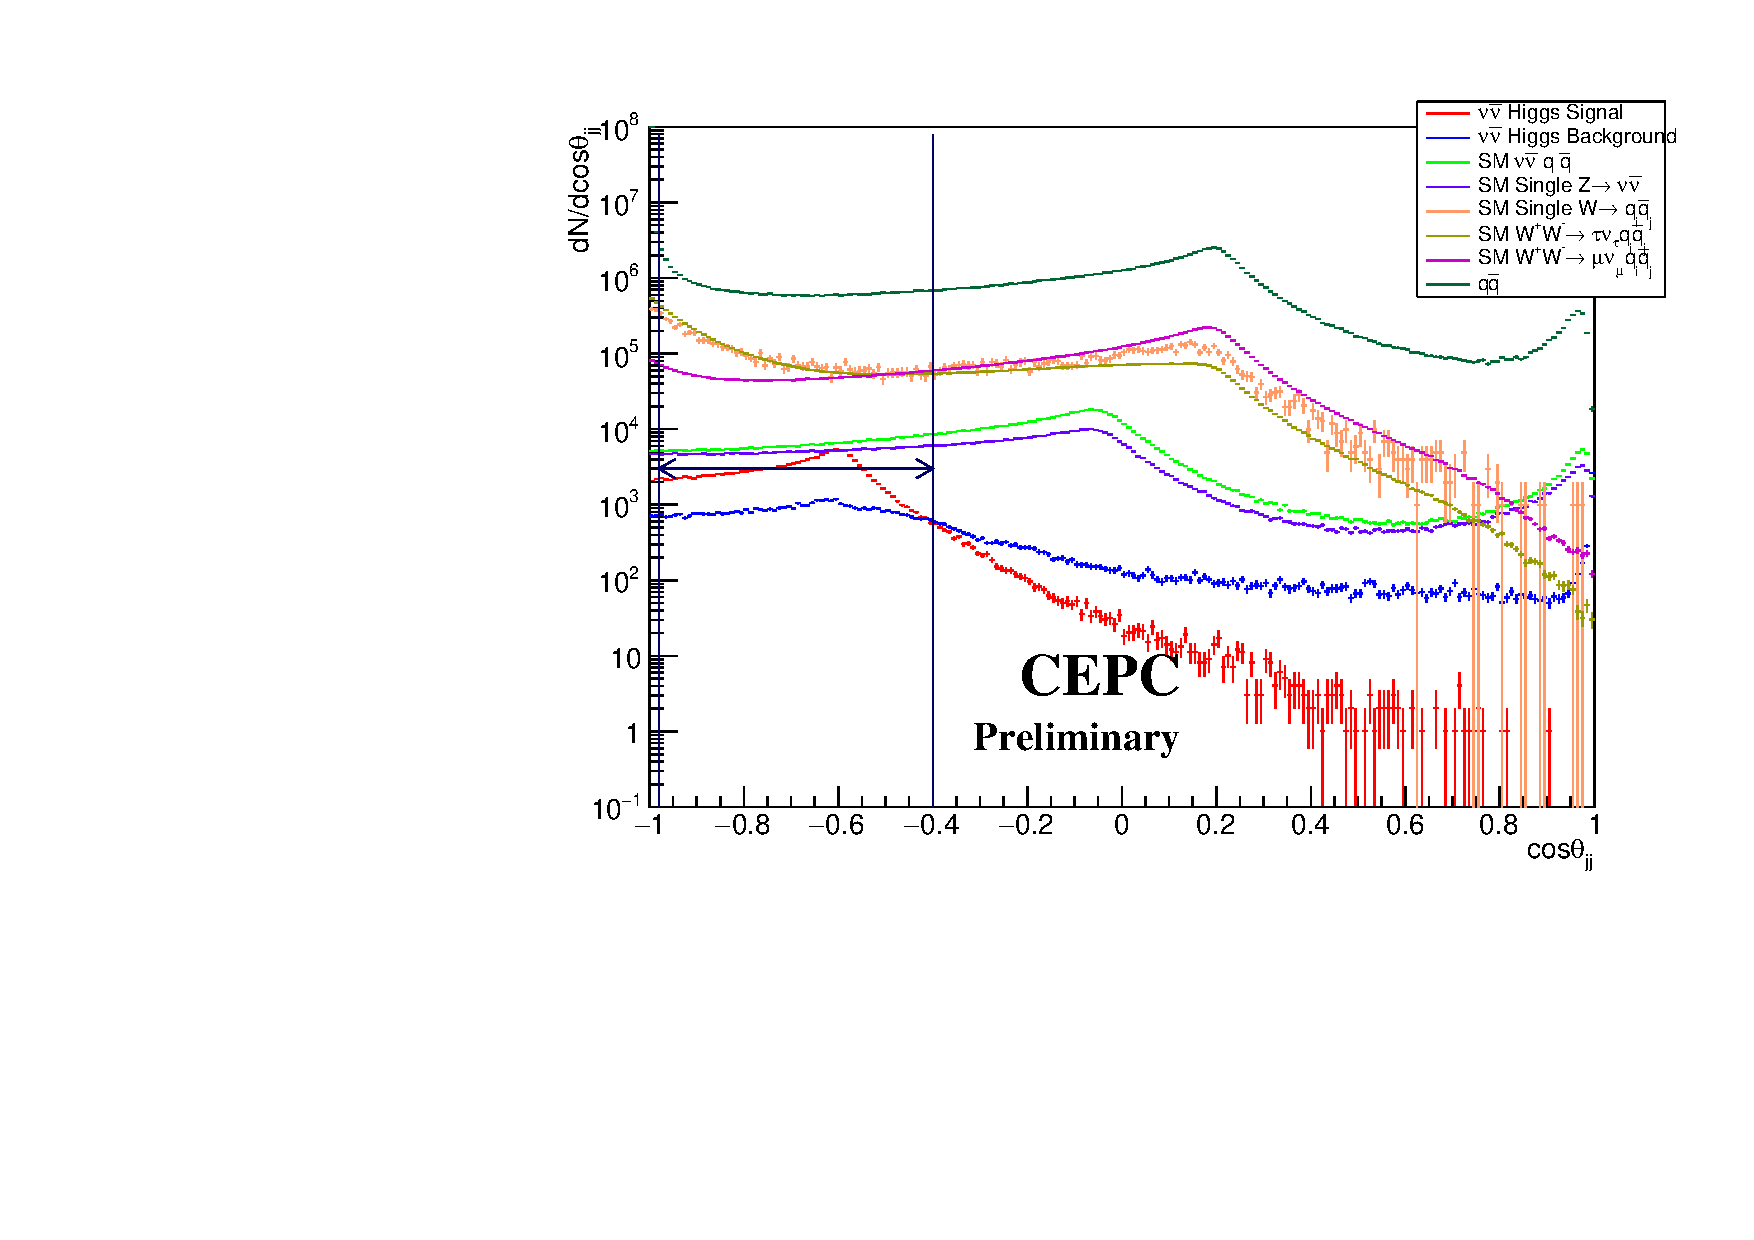
\includegraphics[width=\textwidth]{Analysis/nnh/costheta.pdf}
    \end{minipage}
}
\caption{Visible energy(top left), visible transverse momentum(top middle), jet pair system invariant mass(top right), jet system recoil mass(bottom left) and jet pair system polar angluar(bottom right) distribution in \nnh analysis.}
\end{figure}

\begin{figure}[!htpb]
\label{fig:yth_nnh}
\centering
\subfigure[]
{
  \begin{minipage}[b]{0.31\textwidth}
  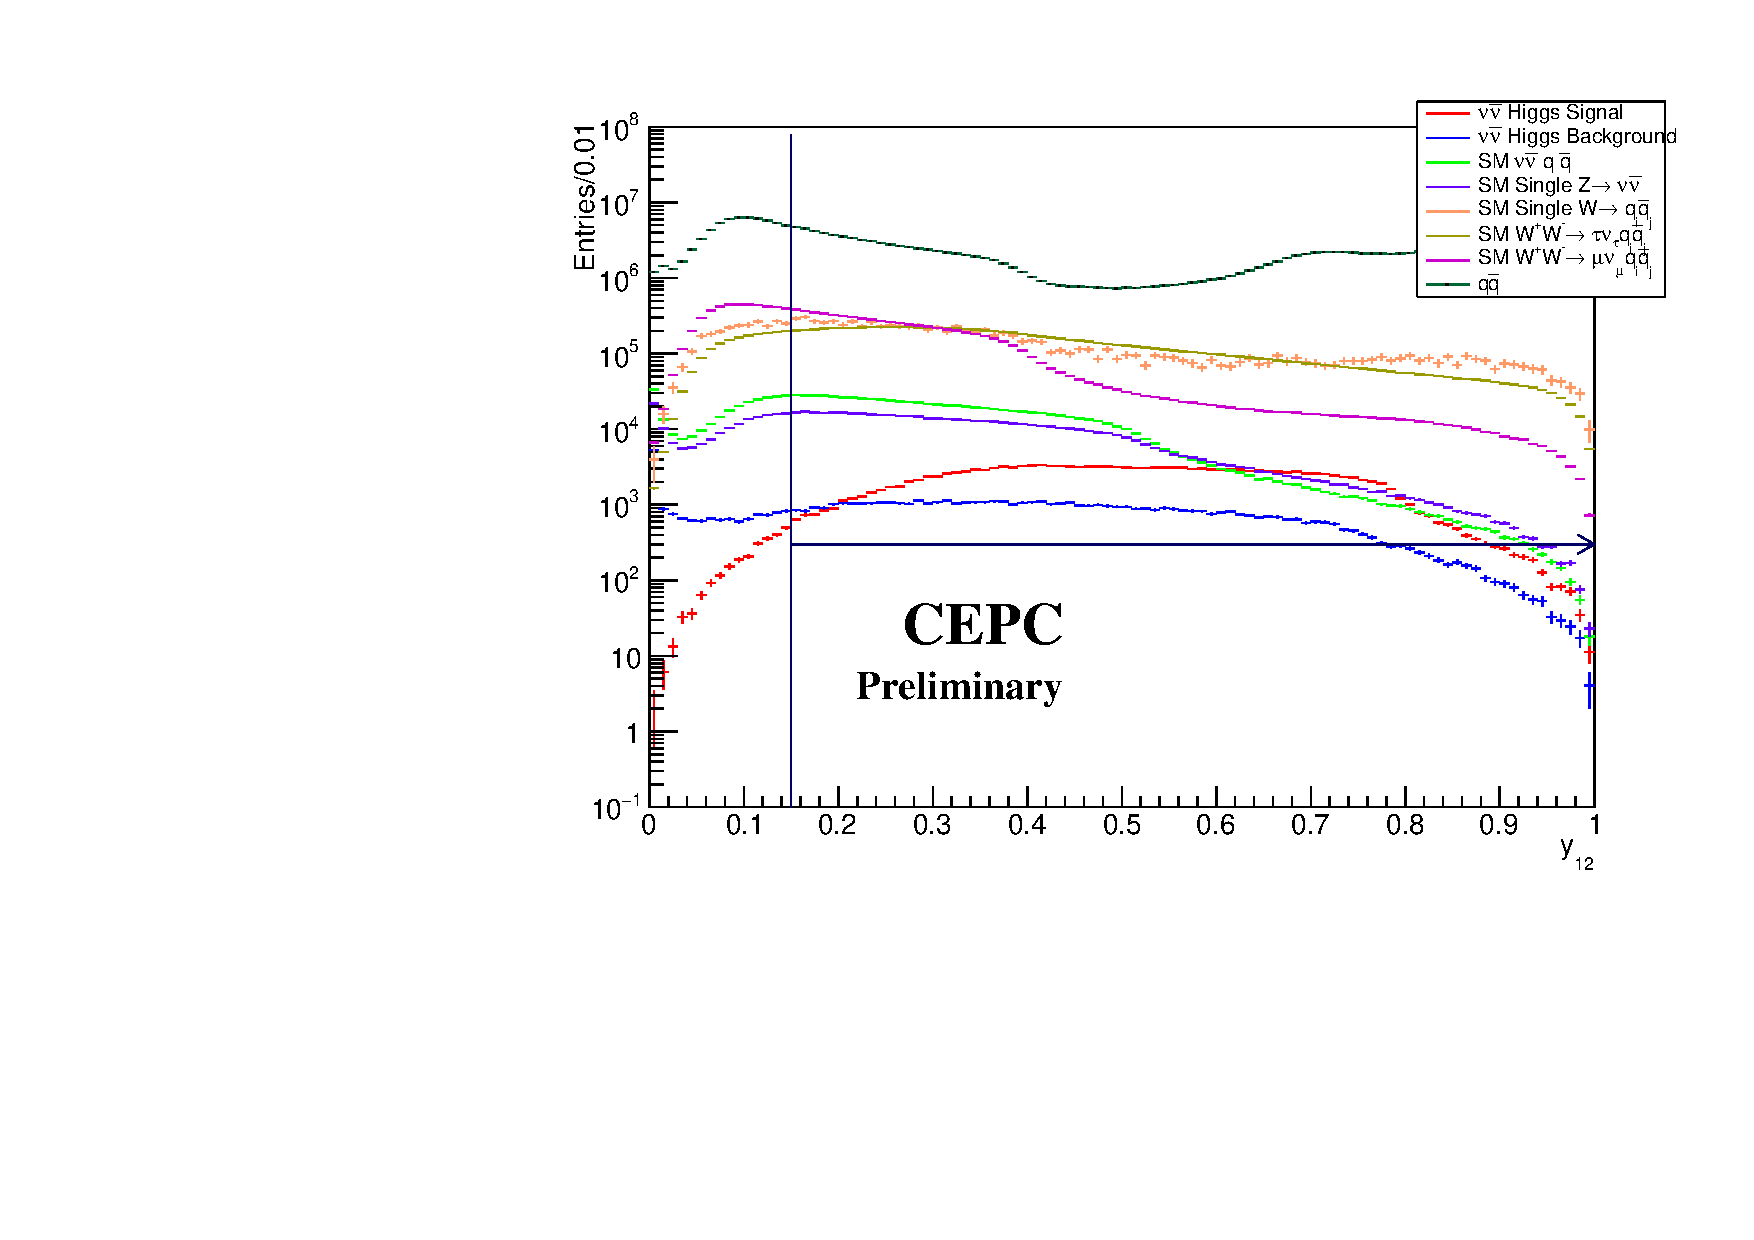
\includegraphics[width=\textwidth]{Analysis/nnh/y12.pdf}
  \end{minipage}   
}
\subfigure[]
{
  \begin{minipage}[b]{0.31\textwidth}
  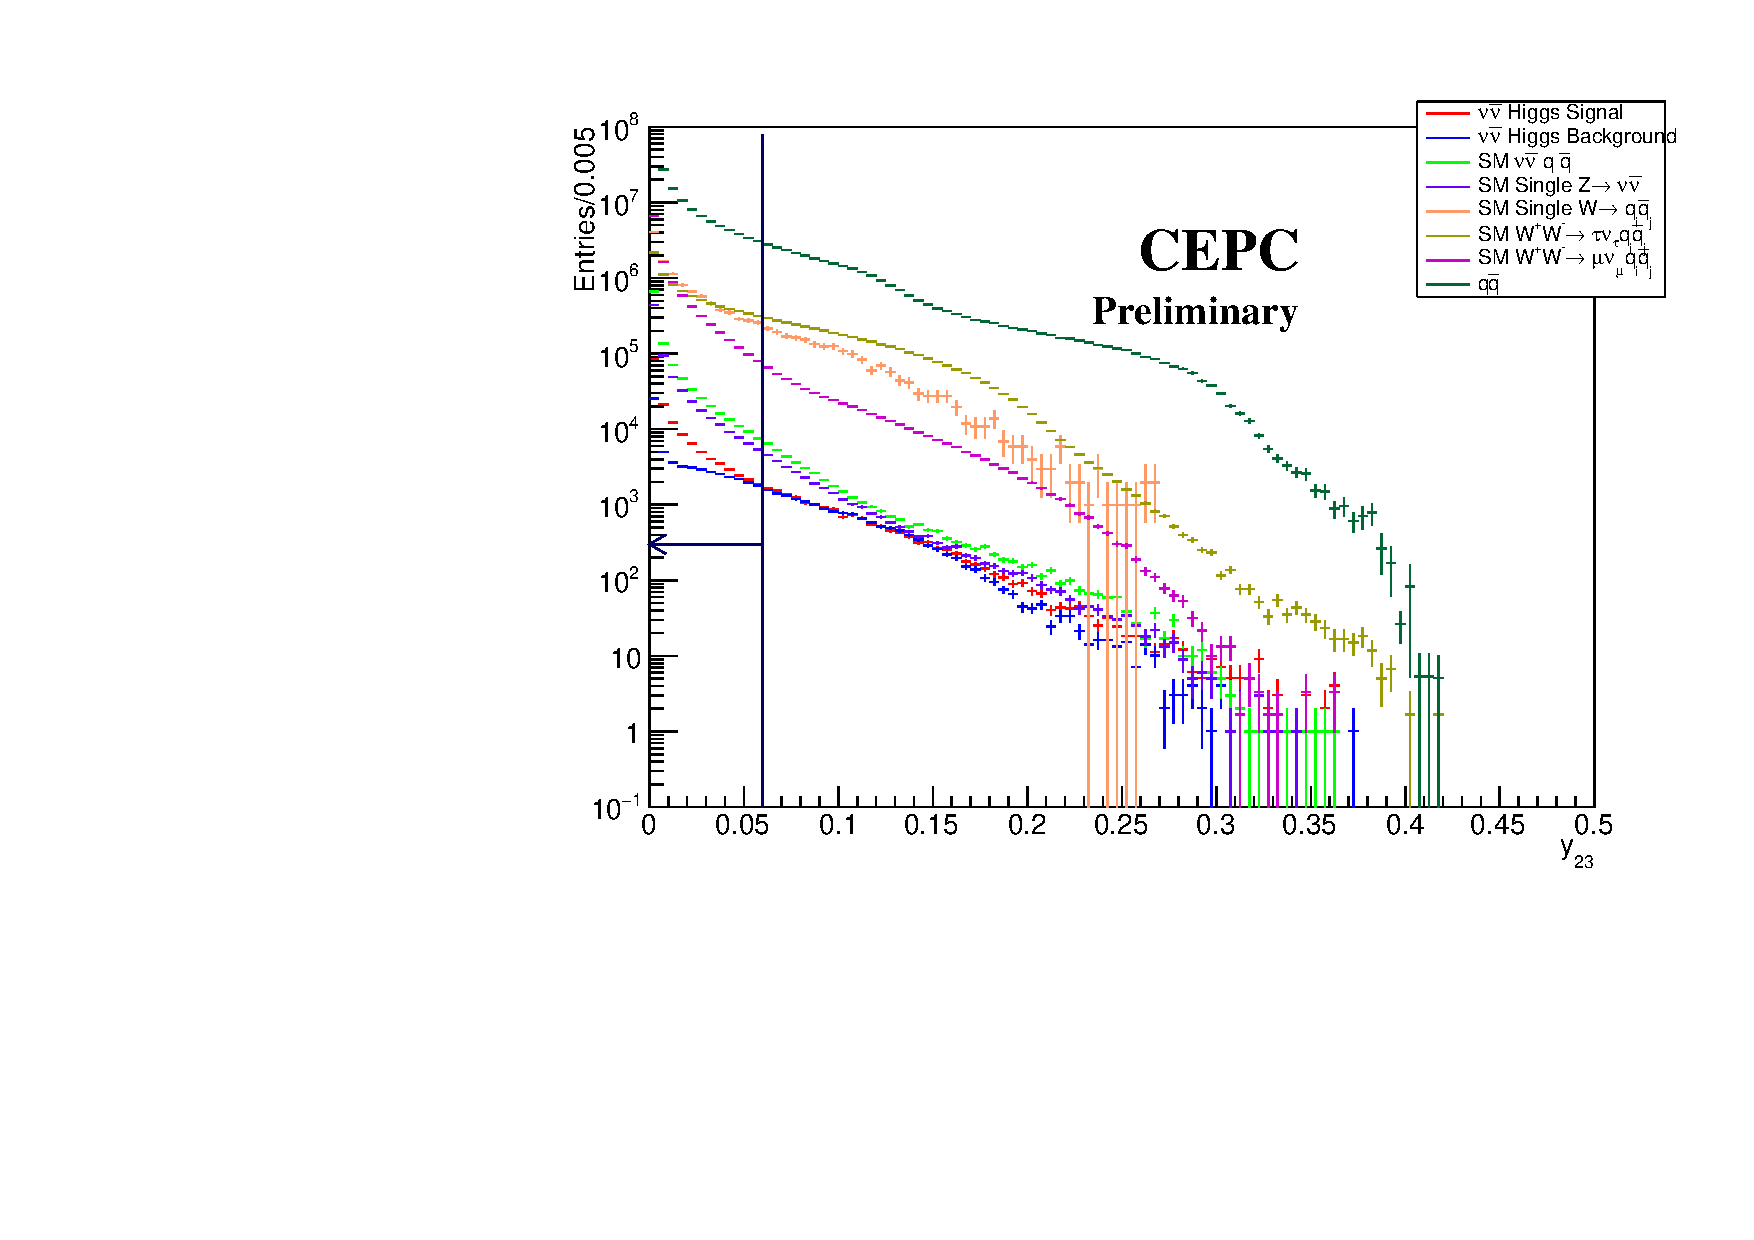
\includegraphics[width=\textwidth]{Analysis/nnh/y23.pdf}
  \end{minipage}
}
\subfigure[]
{
  \begin{minipage}[b]{0.31\textwidth}
  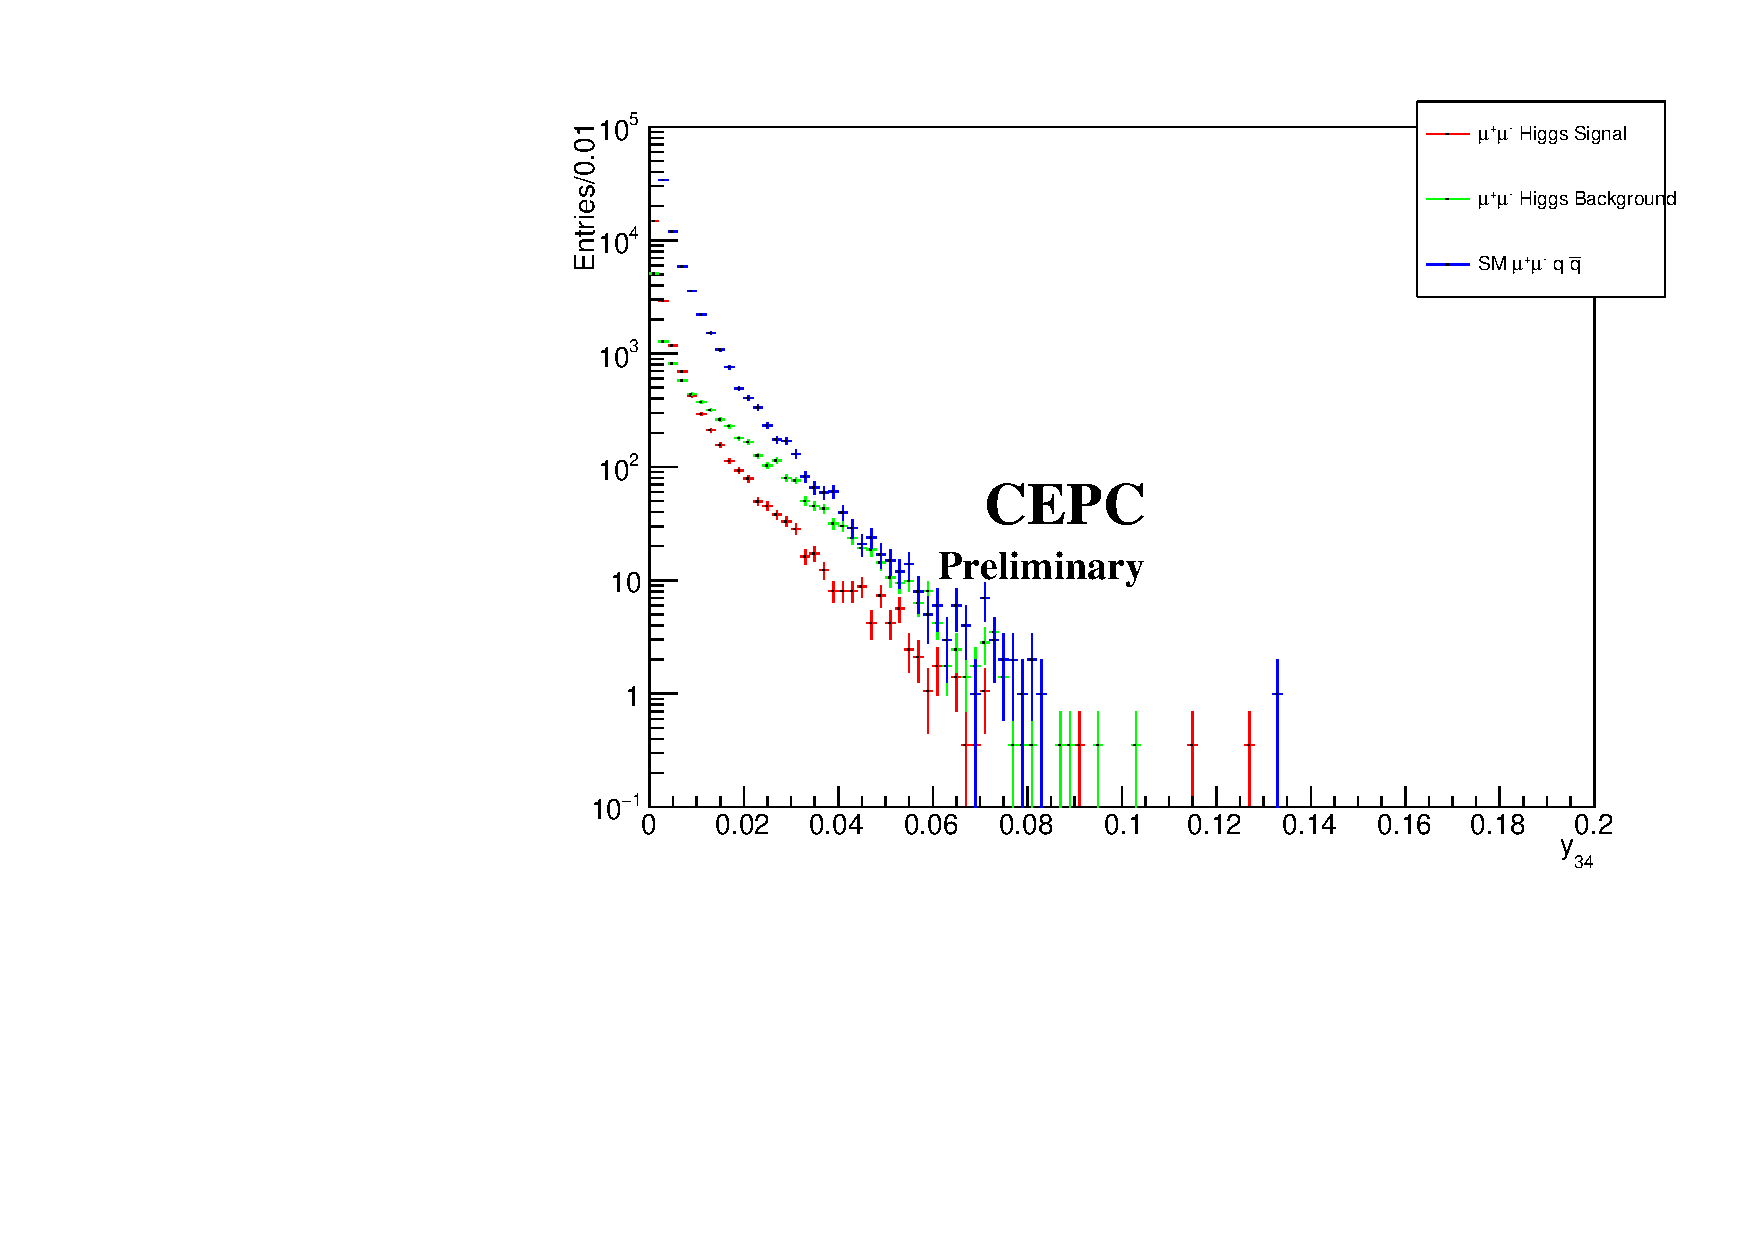
\includegraphics[width=\textwidth]{Analysis/nnh/y34.pdf}
  \end{minipage}
}
\caption{The $y_{12}$(left), $y_{23}$(middle) and $y_{34}$ right distribution in \nnh analysis.}
\end{figure}

\begin{figure}[!htbp]
\label{fig:BDT_nnh}
\centering
\subfigure[]
{
  \begin{minipage}[b]{0.42\textwidth}
  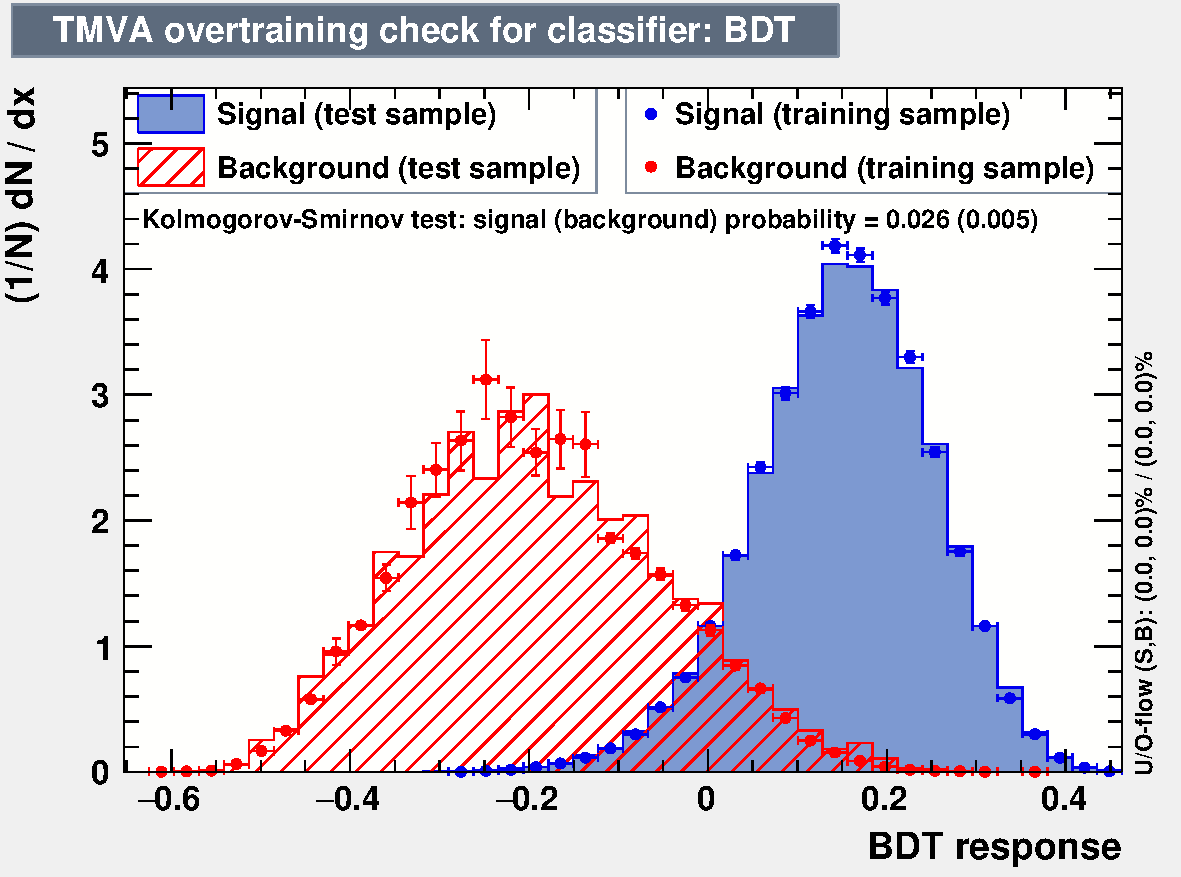
\includegraphics[width=\textwidth]{Analysis/nnh/overtrain_BDT.pdf}
  \end{minipage}   
}
\subfigure[]
{
  \begin{minipage}[b]{0.42\textwidth}
  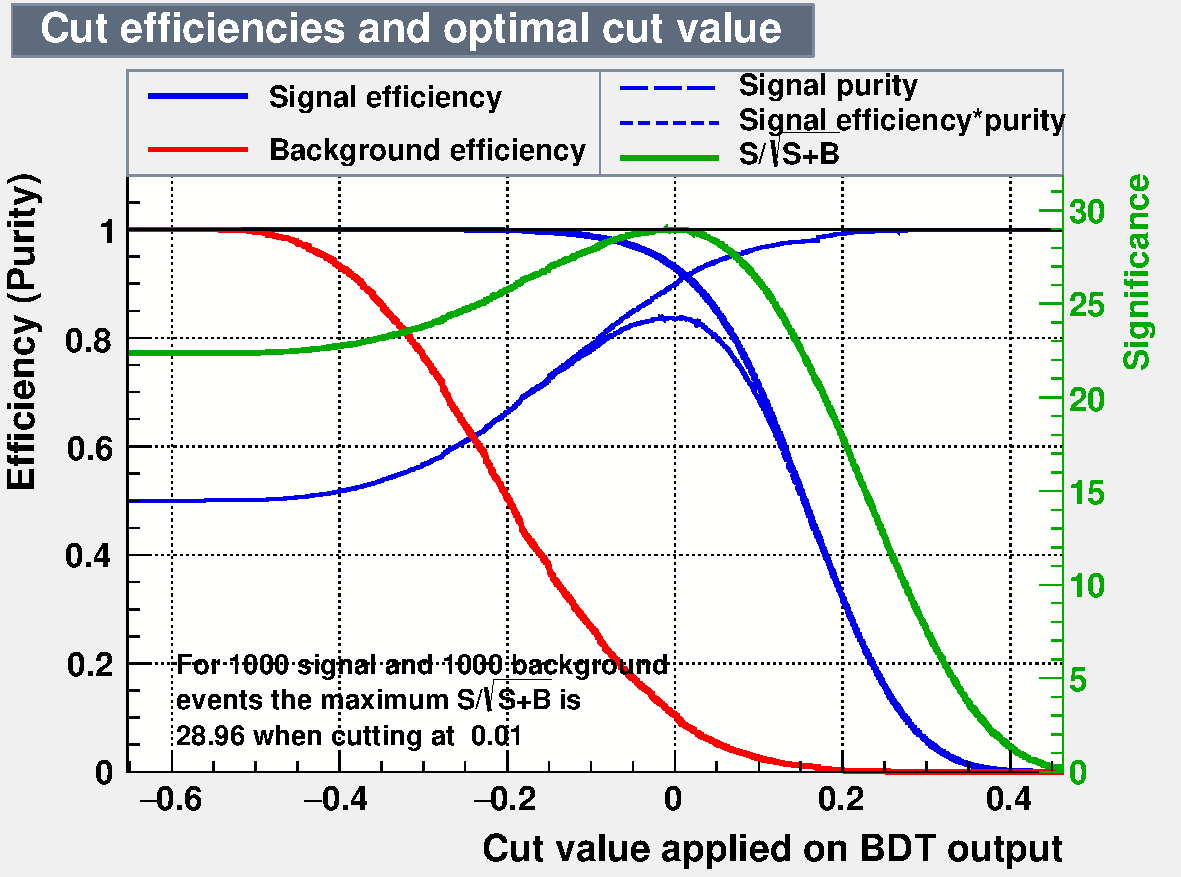
\includegraphics[width=\textwidth]{Analysis/nnh/mvaeffs_BDT.pdf}
  \end{minipage}
}
\caption{Over training check of BDT distribution(left) and optimization of the 
BDT cut performance.}
\end{figure}

\begin{table}[!htbp]
\chuhao
\label{tab:nnh_cut}
\center
\begin{tabular}{c|c|c|c|c|c|c|c|c}\hline
cutflow                 &signal          &\nnh bkg          &zzsl             &sznuqq          &wwsltauq         &wwslmuq           &swslqq           &qq                \\ \hline 
No Cut                  &170633          &76604.1         &\ten{1.08992}{6} &744218          &\ten{1.19114}{7} &\ten{1.19114}{7}  &\ten{1.30255}{7} &\ten{2.46847}{8}  \\ \hline 
2 jets in final state   &170512          &73227.4         &\ten{1.08987}{6} &744201          &\ten{1.19112}{7} &\ten{1.19112}{7}  &\ten{1.30255}{7} &\ten{2.46842}{8}  \\ \hline 
NPFO                    &170349          &42734.8         &980878           &656657          &\ten{1.17604}{7} &\ten{1.16597}{7}  &\ten{1.22262}{7} &\ten{2.39672}{8}  \\ \hline 
$E_{total}$             &152374          &33867.2         &451233           &250618          &\ten{5.06253}{6} &\ten{1.27372}{6}  &\ten{2.07027}{6} &\ten{1.01743}{8}  \\ \hline 
pT                      &142048          &31579.8         &413994           &229568          &\ten{4.31686}{6} &\ten{1.19619}{6}  &\ten{1.93607}{6} &297012            \\ \hline 
IsoLep Veto             &141112          &27966           &410719           &227762          &\ten{3.73815}{6} &365116            &682854           &294929            \\ \hline 
$M_{inv}$               &134583          &26165.2         &41340.5          &23255.3         &\ten{2.20577}{6} &66320             &336493           &111687            \\ \hline 
$M_{recoil}$            &125958          &24817.4         &37889.9          &20720.1         &\ten{1.75479}{6} &29908             &237815           &85653.4           \\ \hline 
y12                     &125228          &24164.8         &37138.4          &20306.8         &\ten{1.61702}{6} &27807.4           &228934           &83451.1           \\ \hline 
y23                     &126365          &13478.1         &29136.3          &15976.7         &\ten{1.07172}{6} &18577.8           &126308           &71353             \\ \hline 
y34                     &107347          &5708.84         &26728            &14616.3         &889531           &16016             &110520           &69372.9           \\ \hline 
costheta                &104023          &5169.31         &21169.6          &11891.4         &506063           &9354.92           &85850.1          &48209.6           \\ \hline 
BDT Cut                 &83852.1         &1961.65         &2704.18          &1566.07         &11116.3          &476.269           &986.783          &6170.45           \\ \hline         
\end{tabular}
\caption{Signal and background yields in the cutflow of \nnh analysis, normalized to 5000 \ifb}
\end{table}

%\clearpage



